\documentclass[preprint,3p,10pt]{elsarticle}
\usepackage[T1]{fontenc}
\usepackage{amsmath,amssymb,booktabs,graphicx,tabularx,array,xcolor,url,microtype,pifont}
\usepackage{tikz}
\usetikzlibrary{arrows.meta,positioning,fit,calc}
\usepackage[colorlinks=true,allcolors=blue!50!black]{hyperref}
\newcommand{\checkmarkx}{\ding{51}}
\renewcommand{\checkmark}{\ding{51}}
\newcolumntype{L}[1]{>{\raggedright\arraybackslash}p{#1}}
\makeatletter\newcommand{\rawinput}[1]{\@@input #1 }\makeatother
\newcommand{\NClinFpLatMax}{164}
\newcommand{\NClinFpN}{21}
\newcommand{\NClinTsLatMax}{2\,990}
\newcommand{\NClinTsLatMaxMs}{2.99}
\newcommand{\NFpEvIdleJitMax}{4\,895}
\newcommand{\NFpEvIdleJitMaxMs}{4.9}
\newcommand{\NFpEvIdleJitOver}{46}
\newcommand{\NFpEvIdleJitPNNN}{181}
\newcommand{\NFpEvIdleLateShare}{50}
\newcommand{\NFpEvIdleMax}{1\,921}
\newcommand{\NFpEvIdleMaxMs}{1.92}
\newcommand{\NFpEvIdleMed}{42}
\newcommand{\NFpEvIdleMiss}{0}
\newcommand{\NFpEvIdleMissPct}{0.00}
\newcommand{\NFpEvIdleN}{7\,161}
\newcommand{\NFpEvIdleNGtOne}{2}
\newcommand{\NFpEvIdleNSamp}{148\,500}
\newcommand{\NFpEvIdlePNNN}{303}
\newcommand{\NFpEvIdlePipeMax}{4\,951}
\newcommand{\NFpEvIdlePipeMaxMs}{5.0}
\newcommand{\NFpEvIdlePipeMiss}{0}
\newcommand{\NFpEvIdlePipeMissPpm}{0}
\newcommand{\NFpEvIdleResMax}{1\,897}
\newcommand{\NFpEvIdleResP}{19}
\newcommand{\NFpEvIdleResPNNN}{78}
\newcommand{\NFpEvIdleUB}{0.042}
\newcommand{\NFpEvStrJitMax}{8\,719}
\newcommand{\NFpEvStrJitMaxMs}{8.7}
\newcommand{\NFpEvStrJitOver}{148}
\newcommand{\NFpEvStrJitPNNN}{984}
\newcommand{\NFpEvStrLateShare}{98}
\newcommand{\NFpEvStrMax}{3\,730}
\newcommand{\NFpEvStrMaxMs}{3.73}
\newcommand{\NFpEvStrMed}{30}
\newcommand{\NFpEvStrMiss}{0}
\newcommand{\NFpEvStrMissPct}{0.00}
\newcommand{\NFpEvStrN}{7\,161}
\newcommand{\NFpEvStrNGtOne}{6}
\newcommand{\NFpEvStrNSamp}{148\,500}
\newcommand{\NFpEvStrPNNN}{625}
\newcommand{\NFpEvStrPipeMax}{10\,800}
\newcommand{\NFpEvStrPipeMaxMs}{10.8}
\newcommand{\NFpEvStrPipeMiss}{1}
\newcommand{\NFpEvStrPipeMissPpm}{7}
\newcommand{\NFpEvStrResMax}{348}
\newcommand{\NFpEvStrResP}{15}
\newcommand{\NFpEvStrResPNNN}{59}
\newcommand{\NFpEvStrUB}{0.042}
\newcommand{\NFpPoIdleJitMax}{4\,932}
\newcommand{\NFpPoIdleJitMaxMs}{4.9}
\newcommand{\NFpPoIdleJitOver}{54}
\newcommand{\NFpPoIdleJitPNNN}{263}
\newcommand{\NFpPoIdleLateShare}{1}
\newcommand{\NFpPoIdleMax}{9\,028}
\newcommand{\NFpPoIdleMaxMs}{9.03}
\newcommand{\NFpPoIdleMed}{3\,020}
\newcommand{\NFpPoIdleMiss}{0}
\newcommand{\NFpPoIdleMissPct}{0.00}
\newcommand{\NFpPoIdleN}{7\,161}
\newcommand{\NFpPoIdleNGtOne}{7161}
\newcommand{\NFpPoIdleNSamp}{148\,500}
\newcommand{\NFpPoIdlePNNN}{5\,113}
\newcommand{\NFpPoIdlePipeMax}{4\,975}
\newcommand{\NFpPoIdlePipeMaxMs}{5.0}
\newcommand{\NFpPoIdlePipeMiss}{0}
\newcommand{\NFpPoIdlePipeMissPpm}{0}
\newcommand{\NFpPoIdleResMax}{5\,466}
\newcommand{\NFpPoIdleResP}{2\,999}
\newcommand{\NFpPoIdleResPNNN}{5\,065}
\newcommand{\NFpPoIdleUB}{0.042}
\newcommand{\NFpPoStrJitMax}{24\,230}
\newcommand{\NFpPoStrJitMaxMs}{24.2}
\newcommand{\NFpPoStrJitOver}{190}
\newcommand{\NFpPoStrJitPNNN}{1\,278}
\newcommand{\NFpPoStrLateShare}{1}
\newcommand{\NFpPoStrMax}{19\,550}
\newcommand{\NFpPoStrMaxMs}{19.55}
\newcommand{\NFpPoStrMed}{3\,018}
\newcommand{\NFpPoStrMiss}{3}
\newcommand{\NFpPoStrMissPct}{0.04}
\newcommand{\NFpPoStrN}{7\,161}
\newcommand{\NFpPoStrNGtOne}{7161}
\newcommand{\NFpPoStrNSamp}{148\,500}
\newcommand{\NFpPoStrPNNN}{6\,021}
\newcommand{\NFpPoStrPipeMax}{24\,444}
\newcommand{\NFpPoStrPipeMaxMs}{24.4}
\newcommand{\NFpPoStrPipeMiss}{8}
\newcommand{\NFpPoStrPipeMissPpm}{54}
\newcommand{\NFpPoStrResMax}{11\,341}
\newcommand{\NFpPoStrResP}{3\,001}
\newcommand{\NFpPoStrResPNNN}{5\,081}
\newcommand{\NFpPoStrUB}{0.108}
\newcommand{\NFpStallMax}{118.0}
\newcommand{\NFpStallMin}{102.0}
\newcommand{\NTestLoadDelta}{-0.519}
\newcommand{\NTestLoadP}{<10^{-300}}
\newcommand{\NTestLoadTsDelta}{0.572}
\newcommand{\NTestLoadTsP}{<10^{-300}}
\newcommand{\NTestPathDelta}{0.999}
\newcommand{\NTestPathP}{<10^{-300}}
\newcommand{\NTestPolicyDelta}{0.991}
\newcommand{\NTestPolicyP}{<10^{-300}}
\newcommand{\NTsEvIdleJitMax}{4\,661}
\newcommand{\NTsEvIdleJitMaxMs}{4.7}
\newcommand{\NTsEvIdleJitOver}{72}
\newcommand{\NTsEvIdleJitPNNN}{369}
\newcommand{\NTsEvIdleLateShare}{69}
\newcommand{\NTsEvIdleMax}{3\,227}
\newcommand{\NTsEvIdleMaxMs}{3.23}
\newcommand{\NTsEvIdleMed}{88}
\newcommand{\NTsEvIdleMiss}{0}
\newcommand{\NTsEvIdleMissPct}{0.00}
\newcommand{\NTsEvIdleN}{7\,161}
\newcommand{\NTsEvIdleNGtOne}{6}
\newcommand{\NTsEvIdleNSamp}{148\,500}
\newcommand{\NTsEvIdlePNNN}{891}
\newcommand{\NTsEvIdlePipeMax}{4\,714}
\newcommand{\NTsEvIdlePipeMaxMs}{4.7}
\newcommand{\NTsEvIdlePipeMiss}{0}
\newcommand{\NTsEvIdlePipeMissPpm}{0}
\newcommand{\NTsEvIdleResMax}{2\,972}
\newcommand{\NTsEvIdleResP}{15}
\newcommand{\NTsEvIdleResPNNN}{106}
\newcommand{\NTsEvIdleUB}{0.042}
\newcommand{\NTsEvStrJitMax}{24\,314}
\newcommand{\NTsEvStrJitMaxMs}{24.3}
\newcommand{\NTsEvStrJitOver}{70752}
\newcommand{\NTsEvStrJitPNNN}{11\,242}
\newcommand{\NTsEvStrLateShare}{99}
\newcommand{\NTsEvStrMax}{12\,772}
\newcommand{\NTsEvStrMaxMs}{12.77}
\newcommand{\NTsEvStrMed}{1\,269}
\newcommand{\NTsEvStrMiss}{17}
\newcommand{\NTsEvStrMissPct}{0.24}
\newcommand{\NTsEvStrN}{7\,161}
\newcommand{\NTsEvStrNGtOne}{3616}
\newcommand{\NTsEvStrNSamp}{148\,500}
\newcommand{\NTsEvStrPNNN}{10\,786}
\newcommand{\NTsEvStrPipeMax}{24\,978}
\newcommand{\NTsEvStrPipeMaxMs}{25.0}
\newcommand{\NTsEvStrPipeMiss}{582}
\newcommand{\NTsEvStrPipeMissPpm}{3919}
\newcommand{\NTsEvStrResMax}{4\,585}
\newcommand{\NTsEvStrResP}{20}
\newcommand{\NTsEvStrResPNNN}{187}
\newcommand{\NTsEvStrUB}{0.356}
\newcommand{\NTsPoIdleJitMax}{10\,633}
\newcommand{\NTsPoIdleJitMaxMs}{10.6}
\newcommand{\NTsPoIdleJitOver}{59}
\newcommand{\NTsPoIdleJitPNNN}{399}
\newcommand{\NTsPoIdleLateShare}{3}
\newcommand{\NTsPoIdleMax}{6\,077}
\newcommand{\NTsPoIdleMaxMs}{6.08}
\newcommand{\NTsPoIdleMed}{3\,070}
\newcommand{\NTsPoIdleMiss}{0}
\newcommand{\NTsPoIdleMissPct}{0.00}
\newcommand{\NTsPoIdleN}{7\,161}
\newcommand{\NTsPoIdleNGtOne}{7159}
\newcommand{\NTsPoIdleNSamp}{148\,500}
\newcommand{\NTsPoIdlePNNN}{5\,167}
\newcommand{\NTsPoIdlePipeMax}{10\,733}
\newcommand{\NTsPoIdlePipeMaxMs}{10.7}
\newcommand{\NTsPoIdlePipeMiss}{1}
\newcommand{\NTsPoIdlePipeMissPpm}{7}
\newcommand{\NTsPoIdleResMax}{5\,994}
\newcommand{\NTsPoIdleResP}{2\,999}
\newcommand{\NTsPoIdleResPNNN}{5\,076}
\newcommand{\NTsPoIdleUB}{0.042}
\newcommand{\NTsPoStrJitMax}{19\,673}
\newcommand{\NTsPoStrJitMaxMs}{19.7}
\newcommand{\NTsPoStrJitOver}{63166}
\newcommand{\NTsPoStrJitPNNN}{9\,774}
\newcommand{\NTsPoStrLateShare}{25}
\newcommand{\NTsPoStrMax}{17\,641}
\newcommand{\NTsPoStrMaxMs}{17.64}
\newcommand{\NTsPoStrMed}{4\,070}
\newcommand{\NTsPoStrMiss}{230}
\newcommand{\NTsPoStrMissPct}{3.21}
\newcommand{\NTsPoStrN}{7\,161}
\newcommand{\NTsPoStrNGtOne}{6778}
\newcommand{\NTsPoStrNSamp}{148\,500}
\newcommand{\NTsPoStrPNNN}{15\,253}
\newcommand{\NTsPoStrPipeMax}{19\,684}
\newcommand{\NTsPoStrPipeMaxMs}{19.7}
\newcommand{\NTsPoStrPipeMiss}{122}
\newcommand{\NTsPoStrPipeMissPpm}{822}
\newcommand{\NTsPoStrResMax}{10\,784}
\newcommand{\NTsPoStrResP}{3\,003}
\newcommand{\NTsPoStrResPNNN}{9\,366}
\newcommand{\NTsPoStrUB}{3.576}
\newcommand{\NTsStallMax}{114.0}
\newcommand{\NTsStallMin}{93.4}
\newcommand{\NWcBui}{23.4}
\newcommand{\NWcCacq}{524.1}
\newcommand{\NWcCacqmean}{1.7}
\newcommand{\NWcCacqpq}{34.2}
\newcommand{\NWcCalarm}{23.3}
\newcommand{\NWcCproc}{67.3}
\newcommand{\NWcCprocmean}{0.6}
\newcommand{\NWcCprocpq}{19.3}
\newcommand{\NWcCwdg}{13.8}
\newcommand{\NWcLmax}{3\,729.9}
\newcommand{\NWcRapp}{652.0}
\newcommand{\NWcShare}{17}
\newcommand{\NWcUtil}{0.1}
\newcommand{\NWcjitmax}{8\,719.4}
\newcommand{\NWcplatform}{3\,077.9}
\newcommand{\NWcresidmax}{348.3}

\newcommand{\NVerTotal}{27}\newcommand{\NVerPass}{27}\newcommand{\NVerFail}{0}
\newcommand{\NHaz}{14}\newcommand{\NReq}{21}\newcommand{\NTraceLinks}{37}
\newcommand{\NHazOpen}{9}
\newcommand{\NHazUnaccInit}{8}
\newcommand{\NHazUnaccRes}{0}
\newcommand{\NFailList}{none}

\journal{(journal to be selected)}

\begin{document}
\begin{frontmatter}
\title{Bounded-latency alarm annunciation in a POSIX real-time patient-monitor simulator: design, hazard-traceable verification, and an empirical comparison of scheduling and alarm-path architectures}

\author[vcet]{M.~Nisha Angeline\corref{cor}}
\cortext[cor]{Corresponding author.}
\address[vcet]{Department of Electronics and Communication Engineering, Velalar College of Engineering and Technology, Thindal, Erode, Tamil Nadu, India}

\begin{abstract}
\textbf{Background and objective.} A physiological alarm is useful only if it is annunciated in time, yet the contribution of software scheduling to alarm delay is rarely specified, measured or traced to a hazard analysis in openly available monitor software. We present an open, portable patient-monitor simulator in which the alarm-system latency is a verified requirement rather than an observed property.
\textbf{Methods.} The simulator acquires synthetic ECG (500\,Hz) and dual-wavelength photoplethysmogram (100\,Hz) signals, detects QRS complexes, estimates SpO$_2$ and raises eight prioritised alarm conditions. It is written against the POSIX real-time interfaces (fixed-priority threads, priority-inheritance mutexes, absolute-time periodic release, locked memory) so that the same source builds for QNX Neutrino and Linux. A hazard log with \NHaz{} hazards is linked to \NReq{} software requirements and \NVerTotal{} automated checks, and is regenerated from executed test results. In a $2\times2\times2$ experiment we compared fixed-priority (FP) against time-sharing (TS) scheduling and an event-driven against a polled alarm path, with and without CPU, memory and I/O overload, using a probe method that timestamps every alarm from the nominal release of the triggering sample to the annunciation output. Measurements were made on a general-purpose Linux kernel in a virtual machine; no QNX measurements are reported.
\textbf{Results.} Under overload, the FP event-driven design had a median alarm latency of \NFpEvStrMed\,\textmu s and a maximum of \NFpEvStrMaxMs\,ms over \NFpEvStrN{} alarms, with \NFpEvStrMiss{} violations of the 10\,ms deadline (95\,\% upper confidence bound on the violation probability \NFpEvStrUB\,\%). The TS event-driven design reached \NTsEvStrMaxMs\,ms and violated the deadline in \NTsEvStrMiss{} of \NTsEvStrN{} alarms (\NTsEvStrMissPct\,\%). Off-target, all detection requirements were met on synthetic signals (asystole time-to-alarm 4.09--4.13\,s over 180 episodes; no false alarm in 4\,h of normal rhythm). \NVerPass{} of \NVerTotal{} checks passed; the failing check(s) (\NFailList) expose platform latency that the application cannot control.
\textbf{Conclusions.} Scheduling policy, not processing cost, dominates alarm-system latency under overload, and an application-level response-time bound accounts for only a small part of the worst observed latency on a virtualised general-purpose kernel. The simulator, its hazard log and the measurement harness are released to support reproduction on real-time operating systems.
\end{abstract}

\begin{keyword}
patient monitoring \sep alarm system \sep real-time operating system \sep POSIX \sep QNX \sep fixed-priority scheduling \sep IEC 62304 \sep hazard analysis \sep electrocardiogram \sep pulse oximetry
\end{keyword}
\end{frontmatter}

\section{Introduction}
Physiological monitors exist to draw attention to a deteriorating patient. The clinical literature on monitor alarms has concentrated, with good reason, on their excess: in one intensive-care study 2.6 million alarms were recorded in 31 days and 88.8\,\% of the annotated arrhythmia alarms were false positives \cite{drew2014}, and the resulting alarm fatigue is a recognised patient-safety problem \cite{cvach2012,clifford2015}. The opposite failure, a true alarm that is produced late or not at all because of the software that carries it, receives less attention but belongs to a well-documented class of defects. Software faults are a leading cause of medical-device recalls \cite{ronquillo2017,alemzadeh2013}, and timing-dependent faults are among the hardest to find by testing, as the Therac-25 accidents showed \cite{leveson1993}.

Alarm timing has two parts. The first is algorithmic: an asystole alarm cannot be raised before the defined pause has elapsed, and a rate alarm needs several beats. The second is the delay added by the computing platform between the moment the data that satisfy the alarm condition are available and the moment the annunciator is driven. IEC~60601-1-8 treats both as alarm-system delays that the manufacturer must determine and disclose \cite{iec6060118}. The platform part is normally small, but on a monitor that also renders waveforms, logs trends, communicates over a network and, increasingly, runs machine-learning inference, it is small only if the software architecture makes it so. Whether it is \emph{bounded} is a property of the scheduler, the synchronisation protocol and the memory policy, and it has to be argued and tested like any other safety requirement \cite{lee2012,hatcliff2014}.

Open research artefacts for medical-device software have focused on other aspects. The generic infusion pump and the pacemaker challenge support formal modelling and verification of control logic \cite{arney2007,kim2011,jiang2012}; OpenICE addresses interoperability \cite{arney2018}; PhysioNet supplies signals and algorithms \cite{goldberger2000,moody2001}. The real-time systems literature provides the scheduling theory \cite{liu1973,joseph1986,audsley1993,sha1990} and careful latency studies of operating systems \cite{cerqueira2013,bristot2020,reghenzani2019,adam2021}, but those studies measure a synthetic wake-up, not the path from a physiological sample to an alarm. We are not aware of an openly available monitor implementation in which the alarm latency is specified as a requirement, linked to a hazard analysis, analysed, and measured end to end under adversarial load.

This paper contributes:
\begin{enumerate}
\item a patient-monitor simulator (ECG and SpO$_2$ acquisition, QRS detection, eight alarm conditions with priorities and latching) written against POSIX real-time interfaces so that one code base targets QNX Neutrino and Linux;
\item a definition of alarm-system latency that separates algorithmic from platform delay, with a probe method that measures it for every alarm without external instrumentation, and an application-level response-time bound;
\item a hazard log in the style of ISO~14971 and IEC~62304 whose links from hazard to risk control, requirement and test are machine-checked, and whose status is regenerated from executed tests, including tests that fail;
\item a controlled comparison of fixed-priority versus time-sharing scheduling and of event-driven versus polled alarm paths, with and without overload, on a general-purpose kernel.
\end{enumerate}

We state the main limitation at the outset. All measurements were taken on a stock Linux kernel running in a virtual machine. They characterise the application architecture and show what such a platform cannot guarantee; they do not characterise QNX or any other real-time operating system, on which the software has been designed to run but has not yet been measured.

\section{Background and related work}
\subsection{Alarm systems and the standards that shape them}
IEC~60601-1-8 defines alarm conditions, three priorities (high, medium, low) with distinct visual and auditory signals, latching and non-latching alarm signals, and the notions of alarm condition delay and alarm signal generation delay \cite{iec6060118}. Particular standards add device-specific requirements: IEC~60601-2-27 for electrocardiographic monitors, including the amplitude range over which QRS complexes must be detected and the time to alarm for rate limits and cardiac standstill \cite{iec60601227}, and ISO~80601-2-61 for pulse oximeters \cite{iso80601261,jubran2015}. IEC~62304 governs the software life cycle and assigns a safety class (A, B or C) according to the severity of harm to which a software failure can contribute; it requires risk control measures implemented in software to be captured as requirements and verified, and the chain from hazardous situation through software item and cause to risk control measure and its verification to be documented \cite{iec62304}. ISO~14971 supplies the risk-management process \cite{iso14971}. Studies of industrial practice report that this traceability is costly to maintain and often incomplete \cite{regan2013}.

\subsection{Real-time scheduling}
Under fixed-priority pre-emptive scheduling the worst-case response time of a task is the fixed point of a recurrence over the execution times of all higher-priority tasks plus a blocking term \cite{joseph1986,audsley1993,buttazzo2011}. Shared resources protected by ordinary mutexes can make the blocking term unbounded (priority inversion); the priority-inheritance protocol bounds it by the length of one critical section per lower-priority task \cite{sha1990}. These results assume that the operating system itself adds a bounded delay between an event and the dispatch of the highest-priority ready thread.

That assumption is what distinguishes operating systems. QNX Neutrino is a microkernel in which drivers, file systems and protocol stacks are user processes that communicate by synchronous message passing, and kernel operations are short and pre-emptible \cite{hildebrand1992}; it implements the POSIX real-time interfaces \cite{posix2017} and is widely used in certified medical and automotive products. Mainline Linux offers the same interfaces (\texttt{SCHED\_FIFO}, priority-inheritance futexes, \texttt{mlockall}, \texttt{clock\_nanosleep}) but, without the \texttt{PREEMPT\_RT} configuration, contains non-pre-emptible sections of unbounded length; with it, scheduling latencies in the tens to low hundreds of microseconds are reported on embedded hardware \cite{reghenzani2019,adam2021}, although I/O-bound background load remains a known source of long tails \cite{cerqueira2013} and sound bounds require analysis of kernel behaviour rather than black-box measurement \cite{bristot2020}. Published comparisons place commercial real-time operating systems, QNX among them, ahead of \texttt{PREEMPT\_RT} in worst-case latency \cite{fayyad2013}.

\subsection{Signal processing for ECG and pulse oximetry}
The Pan--Tompkins algorithm (band-pass filtering, differentiation, squaring, moving-window integration and adaptive dual thresholds) remains the reference real-time QRS detector \cite{pan1985}. Synthetic ECG with controllable morphology and rate can be generated from a sum of Gaussian waves placed around each beat \cite{mcsharry2003}. Pulse oximeters estimate arterial oxygen saturation from the ratio of the pulsatile-to-static absorbance at red and infrared wavelengths, and lose validity at low perfusion \cite{jubran2015}.

\section{System design}
\subsection{Requirements and latency definition}
The simulator implements \NReq{} software requirements (the complete list is part of the released hazard log). Those that matter for timing are:
\begin{itemize}
\item \textbf{SRS-RT-01} The annunciation output shall be driven no later than $D=10$\,ms after the nominal release instant of the sample that makes an alarm condition true, including under CPU, memory and I/O overload from non-critical software.
\item \textbf{SRS-RT-04} The release jitter of the acquisition task shall not exceed 1\,ms (half a sampling period).
\item \textbf{SRS-WDG-01} A stall of acquisition or processing longer than 100\,ms shall raise a high-priority technical alarm within 200\,ms.
\item \textbf{SRS-ALM-01} Asystole shall be annunciated between 4.0\,s and 4.5\,s after the last QRS complex.
\end{itemize}
The 10\,ms budget was fixed before any measurement. It is five sampling periods and 0.25\,\% of the shortest algorithmic delay in the system (the 4\,s asystole criterion), so that platform delay is negligible in the disclosed alarm-condition delay if the budget is met.

Let sample $k$ have nominal release instant $r_k=t_0+kT$ with $T=2$\,ms. For an alarm occurrence let $k^\ast$ be the first sample whose processing makes the alarm condition true and $t_{\mathrm{fire}}$ the instant at which the alarm manager has written to the annunciator. We define
\begin{equation}
L \;=\; t_{\mathrm{fire}} - r_{k^\ast}, \qquad\text{and the algorithmic delay}\qquad A \;=\; r_{k^\ast}-t_{\mathrm{onset}},
\end{equation}
where $t_{\mathrm{onset}}$ is the physiological onset (for asystole, the last R wave). $A$ is a deterministic function of the signal and the algorithm, and is verified off-target at full speed. $L$ depends only on the platform and the software architecture, and includes release jitter, queueing, the execution of acquisition and processing for sample $k^\ast$, and the dispatch and execution of the alarm manager. Referring $L$ to the \emph{nominal} release instant rather than to the instant the acquisition thread actually ran makes a late acquisition count against the budget.

\subsection{Architecture}
\begin{figure}[t]
\centering
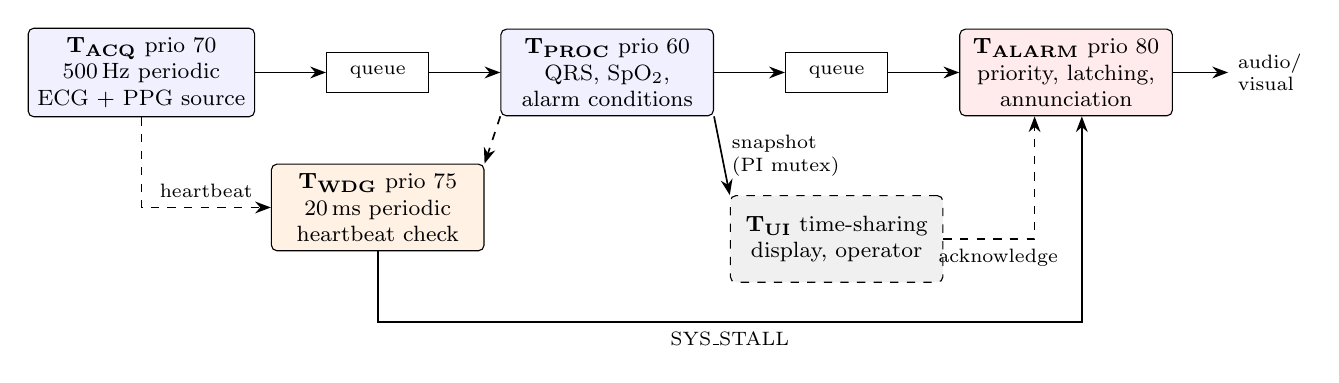
\begin{tikzpicture}[font=\footnotesize, node distance=6mm and 9mm,
  th/.style={draw, rounded corners=2pt, minimum height=11mm, minimum width=27mm, align=center, fill=blue!6},
  nrt/.style={th, fill=gray!12, dashed}, q/.style={draw, minimum height=5mm, minimum width=13mm, fill=white, font=\scriptsize},
  ar/.style={-{Stealth[length=2mm]}, semithick}]
\node[th] (acq) {\textbf{T\textsubscript{ACQ}} prio 70\\500\,Hz periodic\\ECG + PPG source};
\node[q, right=of acq] (q1) {queue};
\node[th, right=of q1] (proc) {\textbf{T\textsubscript{PROC}} prio 60\\QRS, SpO$_2$,\\alarm conditions};
\node[q, right=of proc] (q2) {queue};
\node[th, right=of q2, fill=red!8] (alm) {\textbf{T\textsubscript{ALARM}} prio 80\\priority, latching,\\annunciation};
\node[th, below=9mm of q1, fill=orange!10] (wdg) {\textbf{T\textsubscript{WDG}} prio 75\\20\,ms periodic\\heartbeat check};
\node[nrt, below=13mm of q2] (ui) {\textbf{T\textsubscript{UI}} time-sharing\\display, operator};
\node[right=7mm of alm, align=left, font=\scriptsize] (out) {audio/\\visual};
\draw[ar] (acq) -- (q1); \draw[ar] (q1) -- (proc); \draw[ar] (proc) -- (q2); \draw[ar] (q2) -- (alm); \draw[ar] (alm) -- (out);
\draw[ar, dashed] (acq.south) |- (wdg.west) node[pos=0.75, above, font=\scriptsize] {heartbeat};
\draw[ar, dashed] (proc.south west) -- (wdg.north east);
\draw[ar] (wdg.south) -- ++(0,-9mm) -| node[pos=0.25, below, font=\scriptsize] {SYS\_STALL} ($(alm.south)+(2mm,0)$);
\draw[ar] (proc.south east) -- node[right, font=\scriptsize, align=left] {snapshot\\(PI mutex)} (ui.north west);
\draw[ar, dashed] (ui.east) -| node[pos=0.3, below, font=\scriptsize] {acknowledge} ($(alm.south)-(4mm,0)$);
\end{tikzpicture}
\caption{Thread architecture. Shaded solid boxes are fixed-priority real-time threads (larger number = higher priority); the display thread runs in the time-sharing class. Queues are bounded, their mutexes use priority inheritance (PI), and sending never blocks. In the polled variant the second queue is replaced by a condition table that T\textsubscript{ALARM} reads every 5\,ms.}
\label{fig:arch}
\end{figure}

Fig.~\ref{fig:arch} shows the five threads. Priorities follow criticality along the alarm path rather than rate alone: the alarm manager is highest so that an alarm event is never delayed by the code that produced it or by subsequent samples; the watchdog sits above the two threads it supervises so that a runaway processing thread cannot starve it; acquisition is above processing so that sampling instants are not disturbed by data-dependent processing time. The display thread is deliberately outside the real-time class. It shares one data structure with the processing thread (the waveform snapshot), which is the classic setting for priority inversion and is protected by a priority-inheritance mutex \cite{sha1990}.

Four design rules implement SRS-RT-02 and SRS-RT-03: (i) every buffer and log is allocated before the real-time phase and the process is locked in memory; (ii) real-time threads make no file-system or standard-I/O calls, and results are written after the run; (iii) periodic threads sleep to absolute deadlines on the monotonic clock, so that lateness does not accumulate; (iv) all persistence timers (asystole, desaturation, leads-off) count samples, not clock readings, so that scheduling jitter cannot change an alarm decision. Rules (i) and (ii) are checked automatically by an inspection script on every build of the hazard log.

\paragraph{Alarm path variants} In the \emph{event-driven} path the processing thread sends a message for every change of an alarm condition and the alarm manager blocks in a receive call; the hand-over costs one context switch. In the \emph{polled} path, representative of super-loop designs, the processing thread records changes in a shared table and the alarm manager wakes every $T_{\mathrm p}=5$\,ms to read it; a condition that sets and clears between two polls is still annunciated because set events are sticky.

\subsection{Signal source}
The source replaces the analogue front end and is executed inside the acquisition thread at each release, in place of an ADC read. Each beat is a sum of five Gaussian waves (P, Q, R, S, T) positioned relative to the R instant, in the manner of the morphology used in \cite{mcsharry2003}; P and T positions scale with the square root of the RR interval. RR intervals have 2\,\% beat-to-beat variability. Baseline wander (0.25\,Hz, 0.05\,mV), mains interference (50\,Hz, 0.02\,mV) and Gaussian noise (0.02\,mV rms by default) are added. The photoplethysmogram has unit DC level and a pulsatile component of 2\,\% with a systolic peak and dicrotic wave; the red channel is scaled by the ratio $R=(110-\mathrm{SpO_2})/25$, the textbook linear calibration. A scenario script switches among normal rhythm at a given rate and saturation, asystole (pulse amplitude decays with a 0.5\,s time constant) and leads-off (front-end saturation at $+5$\,mV). The source also records ground truth (R instants, segment boundaries).

\subsection{ECG processing and rhythm alarms}
The detector follows Pan and Tompkins \cite{pan1985} at 500\,Hz: 5--15\,Hz band-pass (two second-order Butterworth sections), five-point derivative, squaring, 150\,ms moving-window integration, local-maximum search with an 80\,ms confirmation interval, signal and noise level estimates with the threshold at the noise level plus one quarter of their difference, a 200\,ms refractory period, T-wave discrimination within 360\,ms, and search-back at half threshold after 1.66 mean RR intervals. Heart rate is the mean of the last four RR intervals. Three departures from the textbook algorithm are risk control measures identified in the hazard analysis (Section~\ref{sec:hazard}):
\begin{itemize}
\item an \emph{absolute threshold floor} equivalent to a QRS of about 0.2\,mV, so that after a pause the adaptive threshold cannot decay into the noise and turn noise peaks into beats (hazard H-01);
\item \emph{exclusion of the T-wave window from search-back}, without which the T wave of the last beat before a pause was accepted as a beat and delayed the asystole alarm by about 0.5\,s, a defect found by the verification suite during development;
\item \emph{saturation handling}: while the input is at the rail the last valid value is held, detection is blanked for 300\,ms after recovery and thresholds are re-learnt over 2\,s, so that a reconnection transient neither produces a beat nor inflates the threshold (hazard H-07).
\end{itemize}
Asystole is declared when no QRS has been accepted for 4.0\,s while the ECG is valid; tachycardia and bradycardia when the four-beat rate is above 150 or below 40\,bpm, with 10 and 5\,bpm hysteresis; leads-off after 0.5\,s of saturation.

\subsection{SpO$_2$ processing}
For each wavelength the DC level is a 3\,s moving average and the AC level the root mean square of the residual over 3\,s; $\mathrm{SpO_2}=110-25R$ with $R$ the ratio of the normalised AC levels. Running sums are recomputed exactly every 3\,s to prevent drift. If the infrared perfusion index is below 0.15\,\% the value is declared invalid, limit alarms are suppressed and, after 3\,s, the low-priority technical alarm \texttt{LOW\_PERF} is raised: without this gate the ratio of two noise levels tends to one and the monitor would display a plausible 85\,\% for a pulseless patient (hazard H-09). \texttt{DESAT} (high priority) requires $\mathrm{SpO_2}<85$\,\% for 5\,s and \texttt{SPO2\_LOW} (medium) $<90$\,\% for 10\,s.

\subsection{Alarm manager and watchdog}
The alarm manager is a pure state machine, separate from all operating-system calls so that it can be unit-tested off-target. Each condition has a fixed priority and latching attribute (Table~\ref{tab:clinical}); high-priority physiological alarms latch until acknowledged, an acknowledgement cannot dismiss a condition that is still present, and the annunciation output always equals the highest priority among active alarms. A scripted operator acknowledges latched alarms 3\,s after their condition ends. The watchdog compares heartbeat counters of the acquisition and processing threads every 20\,ms and raises \texttt{SYS\_STALL} after five consecutive checks without progress. A further technical alarm, \texttt{DATA\_LOSS}, is raised if the sample queue overflows.

\subsection{Portability to QNX Neutrino}
The implementation is about 1\,000 lines of C11 (excluding tests) and uses only interfaces specified by POSIX.1 \cite{posix2017}: \texttt{pthread} scheduling attributes, \texttt{PTHREAD\_PRIO\_INHERIT}, \texttt{clock\_nanosleep} with \texttt{TIMER\_ABSTIME}, \texttt{CLOCK\_THREAD\_CPUTIME\_ID} and \texttt{mlockall}. The single non-portable operation, binding threads to a processor core, is isolated behind a conditional that selects the QNX run-mask call. A cross-build target for the QNX compiler driver is provided. \emph{We have not compiled or run the code on QNX}; the port path is a design property and an invitation to replication, not a result of this paper.

\section{Application-level response-time bound}
\label{sec:rta}
Consider the event-driven path on one core. Let $C_{\mathrm{acq}}$, $C_{\mathrm{proc}}$, $C_{\mathrm{alm}}$ and $C_{\mathrm{wdg}}$ be the worst-case execution times of one job of each thread, $T_{\mathrm{wdg}}=20$\,ms, and $B$ the longest critical section of the display thread on the shared snapshot (the only lower-priority resource user, executed at most once per blocking under priority inheritance). When sample $k^\ast$ is released with no backlog, the alarm is annunciated after the acquisition job, the processing job and one alarm job, possibly pre-empted by the watchdog. The fixed-priority response-time recurrence \cite{joseph1986,audsley1993} gives
\begin{equation}
R_{\mathrm{app}} = B + C_{\mathrm{acq}} + C_{\mathrm{proc}} + m\,C_{\mathrm{alm}} + \left\lceil \frac{R_{\mathrm{app}}}{T_{\mathrm{wdg}}} \right\rceil C_{\mathrm{wdg}},
\label{eq:rta}
\end{equation}
where $m\ge 1$ is the number of alarm conditions that change on the same sample. The alarm latency then satisfies
\begin{equation}
L \;\le\; \Lambda + R_{\mathrm{app}} \quad\text{(event-driven)}, \qquad L \;\le\; \Lambda + R_{\mathrm{app}} + T_{\mathrm p} \quad\text{(polled)},
\label{eq:bound}
\end{equation}
where $\Lambda$ collects everything the application cannot control: timer and interrupt latency, non-pre-emptible kernel sections, and, on a virtual machine, intervals in which the hypervisor does not run the virtual processor. If $R_{\mathrm{app}}<T$ no backlog forms, which justifies the single-sample analysis. On an operating system that guarantees a bound on $\Lambda$, Eq.~\eqref{eq:bound} is a guarantee; elsewhere it separates the part of a measured latency that the architecture explains from the part that it does not. We use it in the second sense, with execution times taken as the maxima observed with the per-thread CPU-time clock, which are measurements and not safe upper bounds.

\section{Hazard log and traceable verification}
\label{sec:hazard}
\begin{table}[p]
\caption{Hazard log (condensed). $R_0$ and $R_1$ are the risk indices (severity\,$\times$\,probability of harm, each rated 1--5) before and after the risk control measures; $\ge 12$ is rated unacceptable, 6--10 tolerable, $\le 5$ acceptable. Requirement and test identifiers omit their \texttt{SRS-} and \texttt{TC-} prefixes. Status is computed from executed tests: \checkmark\ = every linked test passed, \textbf{open} = at least one linked test failed on the evaluation platform. Ratings are illustrative engineering judgements for a simulator, not a clinical risk assessment.}
\label{tab:hazard}
\scriptsize
\setlength{\tabcolsep}{3pt}
\begin{tabularx}{\textwidth}{@{}l L{0.27\textwidth} c X L{0.085\textwidth} L{0.085\textwidth} c c@{}}
\toprule
ID & Hazard: software cause & $R_0$ & Risk control measures & Req. & Tests & $R_1$ & Status\\
\midrule
\rawinput{tables/tab_hazard.tex}
\bottomrule
\end{tabularx}
\end{table}

The hazard analysis was carried out top-down from two harms (delayed or absent response to a life-threatening condition; desensitisation of staff by false alarms) and bottom-up from the software items. It produced \NHaz{} hazards (Table~\ref{tab:hazard}). Following IEC~62304, the probability that a software fault occurs is taken as one, and the probability rating expresses the likelihood that the hazardous situation leads to harm. The alarm path (acquisition, processing, alarm manager, watchdog) is treated as software safety class~C and the display thread as class~B, segregated from the alarm path by scheduling class and priority.

Each hazard is linked to its risk control measures, each measure to one or more requirements, and each requirement to automated tests. The links are data: a script reads the hazard table, the requirement table and the result files written by the test programs, and regenerates the hazard log with a status for every hazard. A requirement whose planned test has no executed result is reported as not run, and a hazard is reported as verified only if every linked test passed in the current results. The report therefore cannot claim more than was executed, and a failing test propagates to the hazards it supports. There are \NTraceLinks{} hazard--requirement--test links.

Tests are of three kinds. \emph{Off-target tests} run the signal source through the same processing and alarm code as the real-time build, at full speed and deterministically, over several hundred episodes with varied seed, rate, amplitude and noise; they verify detection performance, time to alarm, absence of false alarms and alarm-manager logic. \emph{Run-time tests} are evaluated from the measurement campaign of Section~\ref{sec:method} and verify the timing requirements. One \emph{inspection} is automated: a script confirms that the bodies of the real-time threads contain no heap, standard-I/O or sleep calls, that all shared mutexes are created with priority inheritance, and that memory locking is enabled.

The table is deliberately candid about what the controls do not cover: ventricular fibrillation is not classified, a failure of the alarm-manager thread itself needs an external hardware watchdog, and the leads-off and low-perfusion alarms are not escalated when they coincide.

\section{Experimental method}
\label{sec:method}
\subsection{Platform}
Experiments ran on a four-processor x86-64 virtual machine (KVM-based lightweight virtual machine on an Intel Xeon host) with Linux 6.18, configured with dynamic pre-emption but \emph{without} \texttt{PREEMPT\_RT}, GCC 13.3 at \texttt{-O2}. The monitor's five threads were bound to one virtual processor in every configuration so that the uniprocessor analysis of Section~\ref{sec:rta} applies and configurations differ only in the factors under study. The host is shared and outside our control, and light unrelated activity (compilation, analysis scripts) ran on another virtual processor during parts of the campaign. This platform was chosen because it was available, not because it is suitable for a medical device; it is a harsh but informative test of the architecture.

\subsection{Factors}
Three two-level factors were crossed:
\begin{itemize}
\item \emph{Scheduling}: FP = \texttt{SCHED\_FIFO} at the priorities of Fig.~\ref{fig:arch}, priority-inheritance mutexes and locked memory; TS = the default time-sharing class for all threads, ordinary mutexes, no memory locking. Both use the same absolute-time periodic release.
\item \emph{Alarm path}: event-driven or polled at 5\,ms.
\item \emph{Load}: none, or an interference generator with eight CPU-bound threads (twice the number of processors), two threads that repeatedly allocate, touch and free 48\,MB, and one thread that writes and synchronises 16\,MB files, all unpinned in the time-sharing class.
\end{itemize}
Each of the eight combinations was run three times for 100\,s, blocked by repetition.

\subsection{Latency probe}
Clinical alarms are too rare to characterise a latency distribution. In probe runs the source therefore injects four-sample saturation bursts separated by gaps drawn uniformly from 8 to 24 samples, and the leads-off persistence is shortened to three samples. Each burst travels the complete path (acquisition, queue, filtering and detection, condition evaluation, alarm event, alarm manager, annunciator write) and yields one latency $L$, about 2\,400 per run at random phase relative to all periodic activity. The annunciator is a one-byte write to a character device. In addition, the release jitter (actual minus nominal start of each acquisition job), the pipeline latency (completion of processing minus nominal release) and the CPU time of each job were recorded for all 50\,000 samples per run in pre-allocated memory; the first second of each run was discarded.

\subsection{Fault injection and clinical scenario}
To test the watchdog, a busy loop of 400\,ms was injected into the processing thread at five different phases relative to the watchdog period, under overload, for FP and TS scheduling. To confirm that the off-target results hold in real time, a 210\,s clinical scenario (normal rhythm, 10\,s asystole, tachycardia at 180\,bpm, bradycardia at 32\,bpm, desaturation to 80\,\%, 10\,s leads-off, separated by normal rhythm) was run once without load and twice under overload with FP scheduling, and once under overload with TS scheduling.

\subsection{Statistics}
Latency distributions are heavy-tailed, so we report quantiles and maxima rather than means and standard deviations, compare configurations with the two-sided Mann--Whitney test and Cliff's $\delta$ as effect size, and, where no deadline violation was observed in $n$ alarms, give the one-sided 95\,\% Clopper--Pearson upper bound on the violation probability (approximately $3/n$). A measured maximum is a lower bound on the worst case; we do not treat it as a guarantee.

\section{Results}
\subsection{Off-target verification of detection and alarm logic}
All 27 off-target checks passed. Over 96 synthetic records (3.2\,h; 40--180\,bpm; R amplitude 0.55--4.4\,mV) QRS sensitivity was 99.87\,\% (23 of 18\,252 beats missed) and positive predictivity 100\,\%; the worst four-beat heart-rate error was 4.7\,\%. Asystole was annunciated in all 180 episodes, between 4.088 and 4.132\,s after the last R wave, and in all 20 episodes with 0.05\,mV rms noise. When the ECG was reconnected to a patient already in asystole, so that thresholds were learnt on noise alone, the alarm followed within 6.80\,s in all 20 cases. Maximum times to alarm were 2.40\,s for tachycardia, 7.64\,s for bradycardia, 6.98\,s for \texttt{DESAT}, 12.22\,s for \texttt{SPO2\_LOW} and 7.59\,s for \texttt{LOW\_PERF}; leads-off was declared within one sample of the specified 0.5\,s, with no secondary alarm and full detector recovery. SpO$_2$ error was at most 0.7 percentage points over 70--100\,\%. No alarm of any kind occurred in 4\,h of normal rhythm. These figures describe the algorithms on the synthetic source only.

The suite found two defects during development that a demonstration run would not have revealed: the search-back rule accepted the T wave of the last beat before a pause, delaying one asystole alarm in 180 to 4.59\,s (limit 4.5\,s), and the signal source truncated a P wave at the transition into asystole, which the detector counted as a beat. Both were corrected (the first in the detector, the second in the source) and the corresponding checks are retained as regression tests.

\subsection{Alarm latency}
\begin{table}[t]
\caption{Alarm-system latency $L$ in microseconds (three 100\,s runs per configuration). FP: fixed-priority scheduling with priority inheritance and locked memory; TS: time-sharing. Violations are alarms with $L>10$\,ms; the last column is the one-sided 95\,\% upper confidence bound on the violation probability.}
\label{tab:latency}
\small
\begin{tabular}{@{}lrrrrrrrr@{}}
\toprule
Configuration & $n$ & Median & Mean & $P_{99}$ & $P_{99.9}$ & Max & Violations & 95\,\% UB\\
\midrule
\rawinput{tables/tab_latency.tex}
\bottomrule
\end{tabular}
\end{table}

\begin{figure}[t]
\centering
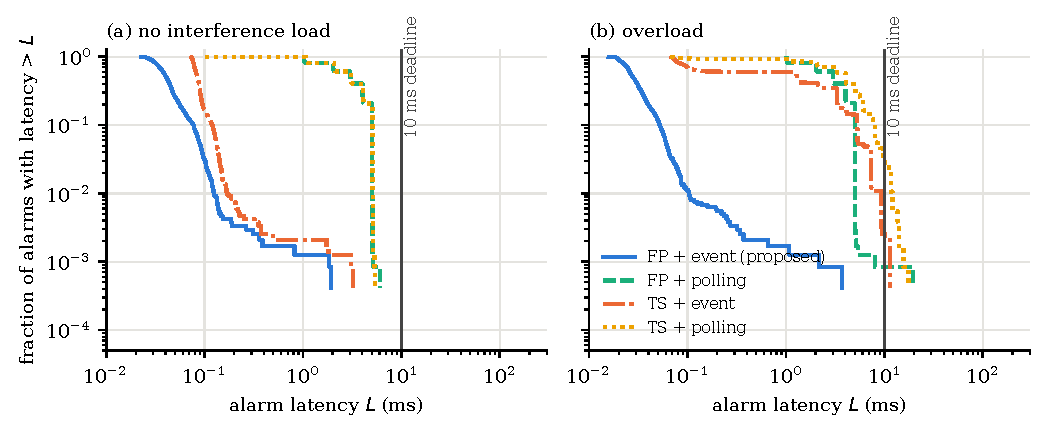
\includegraphics[width=\textwidth]{figs/fig_latency_ccdf.pdf}
\caption{Complementary cumulative distribution of alarm latency for the four architectures, (a) without and (b) with interference load; \NFpEvStrN{} alarms per curve. The plateau of the polled variants reflects the 5\,ms polling period.}
\label{fig:ccdf}
\end{figure}

Table~\ref{tab:latency} and Fig.~\ref{fig:ccdf} summarise \NFpEvStrN{} alarms per configuration. Without load, both event-driven designs had median latencies below 0.1\,ms (\NFpEvIdleMed\,\textmu s for FP, \NTsEvIdleMed\,\textmu s for TS) and no configuration violated the deadline. The polled designs had a median of about 3\,ms and a 99.9th percentile of about 5\,ms, as the polling period predicts.

Under overload the designs separated. With TS scheduling the median latency of the event-driven path rose from \NTsEvIdleMed\,\textmu s to \NTsEvStrMed\,\textmu s, the 99.9th percentile to \NTsEvStrPNNN\,\textmu s, and \NTsEvStrMiss{} alarms (\NTsEvStrMissPct\,\%) violated the deadline; with polling added, \NTsPoStrMiss{} alarms (\NTsPoStrMissPct\,\%) did. With FP scheduling the event-driven path was unaffected in the body of the distribution: the median was \NFpEvStrMed\,\textmu s, the 99.9th percentile \NFpEvStrPNNN\,\textmu s and the maximum \NFpEvStrMaxMs\,ms, with no violation (upper bound \NFpEvStrUB\,\%). The difference between TS and FP event-driven latency under overload was large (Cliff's $\delta=\NTestPolicyDelta$, $p\NTestPolicyP$). The median FP latency was in fact lower under overload than without it (\NFpEvStrMed{} versus \NFpEvIdleMed\,\textmu s, $\delta=\NTestLoadDelta$), which we attribute to the processor not entering an idle state between samples when other threads are runnable.

Fixed-priority scheduling did not, however, make the polled path safe: three of its \NFpPoStrN{} alarms violated the deadline, the worst at \NFpPoStrMaxMs\,ms. Polling consumes half of the 10\,ms budget by construction, so a platform stall of 5\,ms or more, which the next subsection shows does occur, is enough for a violation. The event-driven path keeps almost the whole budget in reserve for such stalls.

\subsection{Release jitter and per-sample pipeline latency}
\begin{table}[t]
\caption{Acquisition release jitter and pipeline latency (nominal release to end of processing) in microseconds over all samples of the probe runs, and the number of samples whose pipeline latency exceeded the 10\,ms alarm budget.}
\label{tab:jitter}
\small
\begin{tabular}{@{}lrrrrrrrr@{}}
\toprule
 & & \multicolumn{3}{c}{Release jitter} & \multicolumn{3}{c}{Pipeline latency} & \\
\cmidrule(lr){3-5}\cmidrule(lr){6-8}
Configuration & Samples & Median & $P_{99.9}$ & Max & Median & $P_{99.9}$ & Max & $>$10\,ms\\
\midrule
\rawinput{tables/tab_jitter.tex}
\bottomrule
\end{tabular}
\end{table}

\begin{figure}[t]
\centering
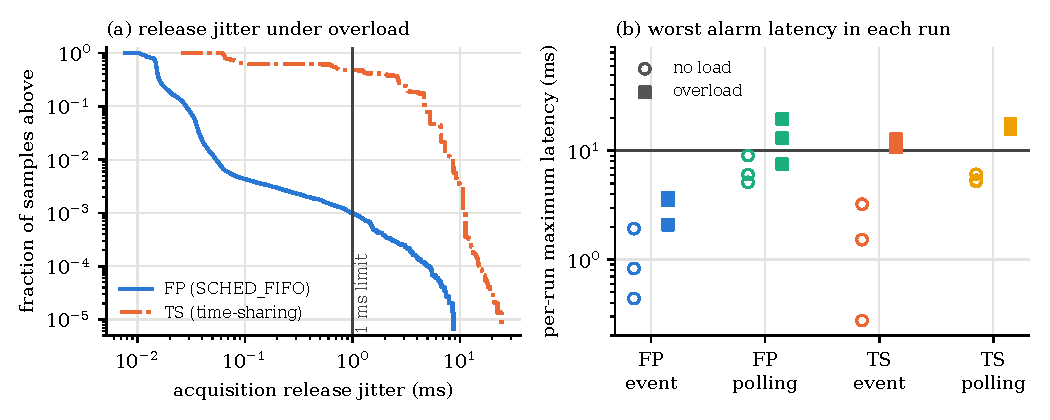
\includegraphics[width=\textwidth]{figs/fig_jitter.pdf}
\caption{(a) Complementary cumulative distribution of acquisition release jitter under overload for fixed-priority and time-sharing scheduling (event-driven path, \NFpEvStrNSamp{} samples each). (b) Largest alarm latency observed in each of the 24 probe runs; the horizontal line is the 10\,ms deadline.}
\label{fig:jitter}
\end{figure}

An alarm can become true on any sample, so the latency of every sample is a stricter test than the latency of the alarms that happened to be injected. Table~\ref{tab:jitter} reports it for \NFpEvStrNSamp{} samples per configuration. Under overload with TS scheduling, \NTsEvStrJitOver{} samples (48\,\%) were released more than 1\,ms late and \NTsEvStrPipeMiss{} (\NTsEvStrPipeMissPpm{} per million) completed processing more than 10\,ms after their nominal release. With FP scheduling the corresponding numbers were \NFpEvStrJitOver{} samples above 1\,ms and \NFpEvStrPipeMiss{} sample above 10\,ms (\NFpEvStrPipeMaxMs\,ms), a reduction by more than two orders of magnitude, but not to zero.

That single sample, and release jitter of up to \NFpEvStrJitMaxMs\,ms at real-time priority (\NFpPoStrJitMaxMs\,ms in the FP polled runs), are the central negative result. Jitter of several milliseconds also occurred without any load (maximum \NFpEvIdleJitMaxMs\,ms, \NFpEvIdleJitOver{} samples above 1\,ms), in a thread that had the highest priority on its processor and nothing to compete with. Requirement SRS-RT-04 (jitter $\le 1$\,ms) therefore failed in every configuration, and the per-sample form of SRS-RT-01 failed for the proposed configuration by one sample in \NFpEvStrNSamp. No sample or alarm event was lost in any run.

\subsection{Measured latency against the application-level bound}
\begin{table}[t]
\caption{Execution times observed with the per-thread CPU-time clock in the proposed configuration under overload, and terms of Eqs.~\eqref{eq:rta}--\eqref{eq:bound}. $C_{\mathrm{wdg}}$ and $B$ come from a supplementary overload run with two additional probes.}
\label{tab:rta}
\small
\begin{tabular}{@{}lr@{}}
\toprule
Quantity & Value (\textmu s)\\
\midrule
$C_{\mathrm{acq}}$: mean / 99.99th percentile / maximum & \NWcCacqmean{} / \NWcCacqpq{} / \NWcCacq\\
$C_{\mathrm{proc}}$: mean / 99.99th percentile / maximum & \NWcCprocmean{} / \NWcCprocpq{} / \NWcCproc\\
$C_{\mathrm{alm}}$: maximum & \NWcCalarm\\
$C_{\mathrm{wdg}}$: maximum & \NWcCwdg\\
$B$ (display critical section): maximum & \NWcBui\\
\midrule
$R_{\mathrm{app}}$ from Eq.~\eqref{eq:rta} with observed maxima, $m=1$ & \NWcRapp\\
Largest $L$ minus release jitter of the triggering sample & \NWcresidmax\\
Largest alarm latency $L$ & \NWcLmax\\
Largest release jitter & \NWcjitmax\\
\bottomrule
\end{tabular}
\end{table}

Table~\ref{tab:rta} places these observations in the terms of Section~\ref{sec:rta}. The mean processor demand of acquisition plus processing was about \NWcCacqmean\,+\,\NWcCprocmean\,\textmu s per 2\,000\,\textmu s period, a utilisation of \NWcUtil\,\%. Observed maxima were two orders of magnitude above the means; maxima of this kind on a virtual machine probably include time in which the thread was charged but not running, and we use them as conservative inputs. They give $R_{\mathrm{app}}=\NWcRapp$\,\textmu s, well inside one sampling period. The supplementary run that supplied $C_{\mathrm{wdg}}$ and $B$ (100\,s, 2\,350 alarms, not included in Table~\ref{tab:latency}) had a larger maximum alarm latency than any campaign run, 7.57\,ms, still without a deadline violation; this illustrates how much an observed maximum depends on the observation window.

To compare with measurement we subtracted from each alarm latency the release jitter of its triggering sample, leaving the time from the actual start of acquisition to annunciation. Under overload this residual had a median of \NFpEvStrResP\,\textmu s, a 99.9th percentile of \NFpEvStrResPNNN\,\textmu s and a maximum of \NWcresidmax\,\textmu s, within $R_{\mathrm{app}}$. Of the \NFpEvStrNGtOne{} alarms with $L>1$\,ms, late release accounted on average for \NFpEvStrLateShare\,\% of the latency. In other words, once the acquisition thread ran, the architecture delivered the alarm within the analysed bound; what the bound does not cover, the term $\Lambda$, was up to \NFpEvStrJitMaxMs\,ms and dominated every long latency. (Without load, two alarms had residuals above $R_{\mathrm{app}}$, up to \NFpEvIdleResMax\,\textmu s, which shows that stalls also strike after release.)

\subsection{Watchdog fault injection}
\begin{table}[t]
\caption{Time from the start of an injected 400\,ms runaway loop in the processing thread to annunciation of \texttt{SYS\_STALL}, under overload (requirement: $\le 200$\,ms).}
\label{tab:stall}
\small
\begin{tabular}{@{}lrrrrr@{}}
\toprule
Configuration & Runs & Undetected & Min (ms) & Mean (ms) & Max (ms)\\
\midrule
\rawinput{tables/tab_stall.tex}
\bottomrule
\end{tabular}
\end{table}
The watchdog detected every injected stall (Table~\ref{tab:stall}), in at most \NFpStallMax\,ms with FP scheduling, consistent with five 20\,ms checks plus up to one period of phase. With FP scheduling the watchdog and alarm manager pre-empt the runaway thread by priority; with TS scheduling detection relied on the fairness of the scheduler and was also timely in these runs, with one detection slightly below 100\,ms because the processing thread had already been starved before the fault was injected.

\subsection{Clinical scenario in real time}
\begin{table}[t]
\caption{Alarms raised in the 210\,s clinical scenario executed in real time: algorithmic delay $A$ from the reference instant, for three runs with FP scheduling (one without load, two under overload; range) and one run with TS scheduling under overload.}
\label{tab:clinical}
\small
\begin{tabular}{@{}llllll@{}}
\toprule
Alarm & Priority & Reference & $A$, FP (s) & $A$, TS (s) & Limit (s)\\
\midrule
\rawinput{tables/tab_clinical.tex}
\bottomrule
\end{tabular}
\end{table}

\begin{figure}[t]
\centering
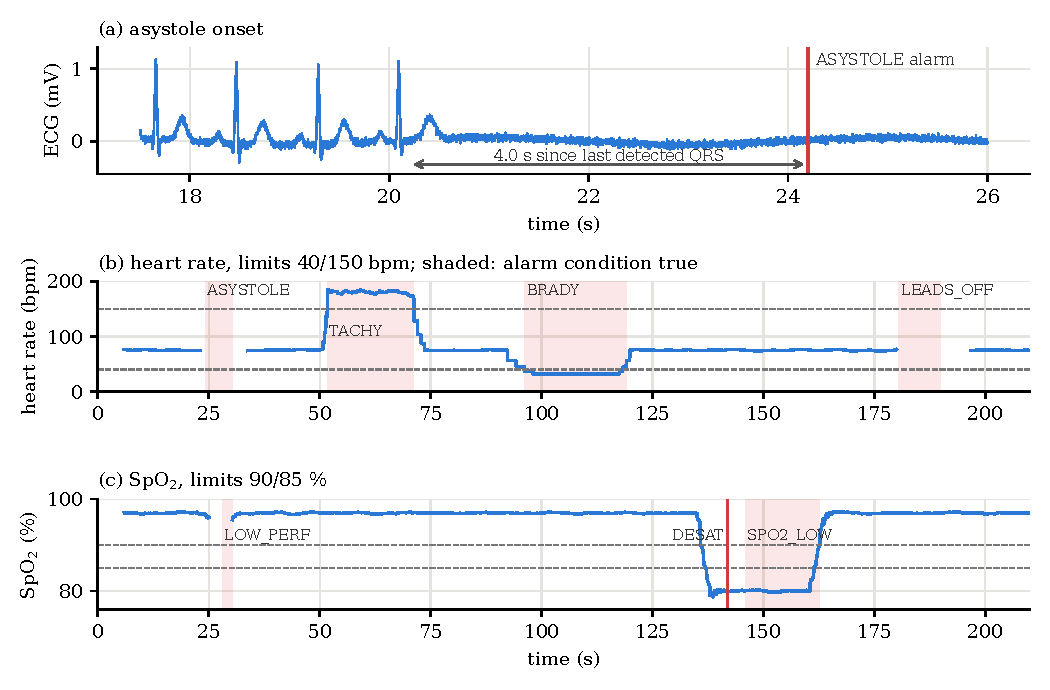
\includegraphics[width=\textwidth]{figs/fig_clinical.pdf}
\caption{Clinical scenario (off-target trace of the same code): (a) ECG at the onset of asystole; (b) heart rate and (c) SpO$_2$ with the intervals in which alarm conditions were true.}
\label{fig:clinical}
\end{figure}

In each real-time run of the clinical scenario exactly the seven expected alarms were raised, once each, with the algorithmic delays of Table~\ref{tab:clinical}; Fig.~\ref{fig:clinical} shows the scenario. Because persistence timers count samples, the TS run raised every alarm on exactly the same sample as the FP run that used the same random seed: scheduling changes when an alarm is annunciated, not whether or on which sample it is raised. The alarm-system latency of the \NClinFpN{} alarms in the FP runs was at most \NClinFpLatMax\,\textmu s; in the TS run under overload it reached \NClinTsLatMaxMs\,ms.

\subsection{Traceability status}
Of the \NVerTotal{} automated checks, \NVerPass{} passed and \NVerFail{} failed (\NFailList). Because status propagates along the links, \NHazOpen{} of the \NHaz{} hazards are reported as open in Table~\ref{tab:hazard}: those whose control depends on bounded alarm latency or on bounded release jitter. All \NHazUnaccInit{} hazards rated unacceptable before controls are rated tolerable or acceptable after them, on the condition that the open items are closed on a platform with a bounded $\Lambda$.

\section{Discussion}
\subsection{What the comparison shows}
Three observations follow from the experiment. First, the cost of the processing itself is irrelevant to alarm latency: QRS detection, SpO$_2$ estimation and alarm evaluation together need about two microseconds per sample on this processor, a utilisation of \NWcUtil\,\%. Any latency problem in a monitor of this kind is a scheduling problem. Second, the scheduling class decides the outcome under overload. With time-sharing, nearly half of all samples were acquired more than a millisecond late and one alarm in four hundred missed a 10\,ms deadline, although the monitor's own demand was negligible; with fixed priorities, priority inheritance and locked memory the body of the latency distribution did not move at all. Time-sharing schedulers optimise fairness and throughput, and a design that relies on them inherits the behaviour of whatever else is installed on the device. Third, the alarm path matters independently of the scheduler. A polled alarm manager spends a fixed part of the budget on waiting, and it was the only fixed-priority variant whose alarms violated the deadline.

\subsection{What a measurement on a general-purpose kernel can and cannot support}
We set out to verify a hard deadline and must report that, on the evaluation platform, we could not. No alarm of the proposed configuration was late, and the upper confidence bound on the violation probability is \NFpEvStrUB\,\%; but one sample in \NFpEvStrNSamp{} was processed after the deadline, and release jitter reached \NFpEvStrJitMaxMs\,ms. Had an alarm condition become true on that sample, the requirement would have been violated. The decomposition of Table~\ref{tab:rta} locates the cause outside the application: the time from the actual start of acquisition to annunciation stayed within the analysed bound, and long latencies were explained by late release. The same stalls appeared without load, which points to the hypervisor and the non-real-time kernel rather than to the interference threads. The guest kernel's own accounting supports the first explanation: it reported about 45\,s of processor time stolen by the hypervisor, summed over the four virtual processors, during the hour of the campaign. We cannot apportion individual stalls between hypervisor and kernel with the instrumentation used here.

This is the argument for a real-time operating system, stated as a measurement rather than as an assumption. The application-level bound $R_{\mathrm{app}}$ becomes a guarantee only when the platform term $\Lambda$ is bounded by construction and by evidence from the supplier, which is what a microkernel such as QNX Neutrino \cite{hildebrand1992}, or \texttt{PREEMPT\_RT} with a kernel-level analysis \cite{bristot2020}, is meant to provide. Our results neither confirm nor quantify that for QNX. They do show that the software is ready for the experiment: the same binaries, scripts and hazard log will report, on a bare-metal real-time target, whether the open items close. We regard the fact that the generated hazard log currently reports \NHazOpen{} open hazards as a feature of the method. A traceability report assembled by hand after the fact would very likely have recorded the zero late alarms and passed.

\subsection{Hazard-driven design}
The hazard analysis changed the software in ways that functional testing alone would not have prompted. The threshold floor, the exclusion of the T-wave window from search-back, the perfusion gate on SpO$_2$ and the re-learning after lead reconnection are each a response to a specific hazardous situation, and each has a test that fails without it. The reverse also held: a verification test for one hazard (asystole time-to-alarm) exposed a defect in a mechanism introduced for another purpose (search-back for missed beats). Keeping the links as data and regenerating the report from executed results cost a few hundred lines of script and addresses the maintenance problem reported for traceability in practice \cite{regan2013}, at least at this scale.

\subsection{Limitations}
\begin{itemize}
\item \emph{Platform.} All timing results come from a virtualised, non-real-time Linux kernel on a shared host, with light unrelated activity on another virtual processor during the campaign. Absolute values will not transfer to other hardware. No measurement was made on QNX; the port has not been compiled.
\item \emph{Duration.} Each configuration was observed for 300\,s. Worst-case behaviour of an operating system emerges over hours or days and under a wider range of loads (interrupt storms, network traffic, storage errors); the maxima reported here are lower bounds on the worst case.
\item \emph{Timing source.} Latencies were measured with the system's own monotonic clock. A stall that also stops the clock source, or an error in the annunciator device itself, is invisible; an external logic analyser on a hardware output is the appropriate reference.
\item \emph{Execution times.} $C$ values are observed maxima, not results of static worst-case execution-time analysis, and include virtualisation artefacts.
\item \emph{Signals and algorithms.} The ECG and photoplethysmogram are synthetic and free of motion artefact, ectopy, pacing and morphology changes; detection figures say nothing about performance on patients. Ventricular fibrillation and tachycardia are not classified, there is one ECG lead, and the SpO$_2$ calibration is the textbook linear curve. Evaluation on annotated databases \cite{goldberger2000,moody2001,clifford2015} is required before any clinical claim.
\item \emph{Alarm system.} Audio pause, alarm limits configurable by the operator, distributed alarm systems and the human factors of annunciation are not implemented. A single-core analysis was used; multi-core deployments need partitioned or global analysis.
\item \emph{Risk analysis.} The hazard log was produced by engineering judgement without clinical or regulatory review. It illustrates a method and is not a risk-management file.
\end{itemize}

\subsection{Future work}
The immediate next step is to repeat the campaign unchanged on QNX Neutrino and on a \texttt{PREEMPT\_RT} kernel on the same single-board computer, with an external timing reference and runs of at least 24\,h, and to replace the synthetic source by replay of annotated recordings. The thread structure also offers a natural place for computationally heavy, non-critical analysis such as learned ECG interpretation or language-model summarisation of alarm context: in the time-sharing class next to the display thread, where the present results indicate that it cannot delay the alarm path provided the scheduling and synchronisation rules of Section~3 are kept. Quantifying that isolation with a realistic inference workload is a direct extension of the overload experiment.

\section{Conclusion}
We built a patient-monitor simulator in which the software contribution to alarm delay is defined, analysed, linked to a hazard log and measured for every alarm. On a general-purpose kernel under CPU, memory and I/O overload, fixed-priority scheduling with an event-driven alarm path kept the median alarm latency at \NFpEvStrMed\,\textmu s and all \NFpEvStrN{} alarms within the 10\,ms deadline, where the time-sharing equivalent violated it in \NTsEvStrMissPct\,\% of alarms and a polled fixed-priority design in three. The same measurements show that the platform, not the application, sets the worst case: one sample in \NFpEvStrNSamp{} exceeded the budget and release jitter reached \NFpEvStrJitMaxMs\,ms, so the corresponding requirements are reported as failed and their hazards as open. The released code, hazard log and measurement harness allow that verdict to be re-evaluated on a real-time operating system without modification.


\section*{Declaration of competing interest}
The author declares no competing interests.

\section*{Funding}
This research received no specific grant from any funding agency.

\section*{Data and code availability}
The complete source code, hazard log, requirement tables, measurement scripts, raw measurement files and the scripts that generate every table and figure in this paper are available in the project repository (URL to be inserted at submission).

\section*{Declaration of generative AI and AI-assisted technologies}
During the preparation of this work the author used an AI coding assistant (Claude, Anthropic) to draft software, run the experiments and analysis, and draft the manuscript text. The author reviewed and edited the content as needed and takes full responsibility for the content of the publication. \emph{(To be revised by the author to reflect the final division of work, in line with the target journal's policy.)}

\bibliographystyle{elsarticle-num}
\bibliography{refs}
\end{document}
